\documentclass[12pt]{article}
\addtolength{\oddsidemargin}{-.875in}
	\addtolength{\evensidemargin}{-.875in}
	\addtolength{\textwidth}{1.75in}

	\addtolength{\topmargin}{-.875in}
	\addtolength{\textheight}{1.75in}
\usepackage{epsfig}
\usepackage{graphicx}
\usepackage{amsthm, amsmath}
\usepackage{amsfonts}
\usepackage{color}
\usepackage{xcolor}
\usepackage{enumitem}

\definecolor{ltgray}{gray}{0.8}

%\numberwithin{equation}{section}

\newcommand{\field}[1]{\mathbb{#1}}
\newcommand{\R}{\field{R}}
\newcommand{\F}{\field{F}}
\newcommand{\p}{\field{P}}
\newcommand{\N}{\field{N}}
\newcommand{\Z}{\field{Z}}
\newcommand{\X}{\field{X}}
\newcommand{\E}{\field{E}}
\newcommand{\W}{\field{W}}
\newcommand{\B}{\field{B}}

\def\qed{\hfill$\diamondsuit$}
\def\II{I\negthinspace I}
\def\B{I\negthinspace\negthinspace B}
\def\ccirc{\negthinspace\circ}
\def\median{\mathop{\mbox{med}}}
\def\argmax{\mathop{\mbox{argmax}}}
\def\argmin{\mathop{\mbox{argmin}}}
\theoremstyle{Conjecture}
\theoremstyle{example}
\theoremstyle{remark}
\theoremstyle{lemma}
\theoremstyle{definition}
\theoremstyle{corol}
\theoremstyle{proposition}
\theoremstyle{condition}
\newtheorem{theorem}{Theorem}
\newtheorem{example}{Example}
\newtheorem{remark}{Remark}
\newtheorem{lemma}{Lemma}
\newtheorem{definition}{Definition}
\newtheorem{corol}{Corollary}
\newtheorem{condition}{Condition}
\newtheorem{proposition}{Proposition}
\newtheorem{Conjecture}{Conjecture}


\def\cod{\stackrel{\cal D}{\longrightarrow}}
\def\cop{\stackrel{\cal P}{\longrightarrow}}
\def\eqd{\stackrel{\cal D}{=}}
\def\eqp{\stackrel{\cal P}{=}}
\def\ap#1{\smash{\mathop{\approx}\limits^{#1}}}
\def\lf{\lfloor}
\def\rf{\rfloor}
\def\lc{\lceil}
\def\rc{\rceil}
%\def\N{{\open N}}
%\def\Z{{\open Z}}

\oddsidemargin -0pt
\evensidemargin -0pt
\topmargin -20pt
\textheight 630pt
\textwidth 460pt
\renewcommand{\baselinestretch}{1.3}
\begin{document}

\bibliographystyle{plain}

\begin{center}
\begin{large}
STAT 380 Final Exam, Spring 2017\\ Instructor: M. Haran,  Penn State University
\end{large}
\end{center}
\begin{flushleft}
NAME:
\end{flushleft}
I have neither given nor received any assistance in the taking of this exam. \\\\
Signature: \\\\
\rule{\textwidth}{1pt}
Instructions: 
\begin{enumerate}
\item This is a closed book exam. 
%You are only allowed one 8.5 inch$\times$11 inch sheet of notes and a calculator.
%\item Please show all your work and write clearly for full credit.
%\item `Box' your final answer to each question (draw a box around it).
% \item You may leave your answer unsimplified,e.g. $0.7^{4}
% \frac{18!}{4!8!}, 14 e^{-23}, 1.67-0.938$.
\item {\it Turn off all electronic devices}! You will be asked to
  leave if your electronic device rings, vibrates, or makes any sound during 
the exam. 
\item Please verify that your exam paper contains all 10 questions.
% \item You may use a calculator and one sheet of notes.  You may
% {\it not} use any books or share a calculator with another student.
%\item Illegible handwriting will not be graded!
\item To earn credit, write clearly, and show your work. When in
  doubt, explain things clearly. If you need extra paper then please write on
  the back of your paper.
% \item {\it The instructors or teaching assistants will answer no
% questions during the exam period.}  Simply explain any error
% you may find in a question and proceed to the next question.
\end{enumerate}
\centerline{DO NOT WRITE BELOW THIS LINE}

\vskip 0.1truein

\begin{table}[!h]
\centering
\begin{tabular}{|c|c|c|}\hline
Question & Marks & Max\\ \hline
1 &  & 8\\ \hline
2 &  & 12\\ \hline
3 &  & 6\\ \hline
4 &  & 14\\ \hline
5 &  & 12\\ \hline
6 &  & 10\\ \hline
7 &  & 6\\ \hline
8 &  & 12\\ \hline
9 &  & 12\\ \hline
10 &  & 8\\ \hline
Total &  & 100\\ \hline
\end{tabular}
\end{table}


\newpage 

%SHORT ANSWERS
\begin{enumerate}

%% Cross validation; logistic regression and CART
\item[Q1] Suppose you have 1000 emails, of which 600 are spam and 400
  are non-spam (``ham''). The goal is to develop a classification
  method based on these emails for classifying spam versus ham
  emails. Your friend has an approach that fits a logistic regression
  based on several characteristics of these emails. Call this Method
  A. You want to use a naive Bayes approach (using ``bag of words'' as
  capturing the email characteristics) that fits and predicts spam
  versus ham. Call this Method B. Describe clearly {\it in around 5
    sentences/steps} how you would use cross-validation to determine
  whether you prefer Method A or Method B. No code necessary, but if
  you are vague in your description you will lose points.  [8 pts]

{\color{blue}
\begin{itemize}
	\item Randomly split the data into 10 groups of 100 emails each.
	\item Using each method, train a model on the first 9 groups and test it on the tenth group. Record the number of incorrectly classified emails for each model, call them $\textrm{Err}^A_1$ and $\textrm{Err}^B_1$.
	\item Repeat the previous step, testing on a different group each time, until you have $\textrm{Err}^A_1, \dots, \textrm{Err}^A_{10}$ and $\textrm{Err}^B_1, \dots, \textrm{Err}^B_{10}$.
	\item The cross-validated misclassification rate for each method is the average of these values. $CV_A = \frac{1}{10}\sum_{i=1}^{10} \textrm{Err}^A_i$ and $CV_B = \frac{1}{10}\sum_{i=1}^{10} \textrm{Err}^B_i$.
	\item Choose the method with the smaller cross-validated misclassification rate.
\end{itemize}
}
\newpage

%% database queries/SQL
\item [Q2] Consider the chips database discussed in lecture about CPU
  (central processing unit) development of PCs (personal computers)
  over time. The database has the following variables (column):
  processor, date, transistors, microns, clockspeed, width,
  mips. Write SQL queries to do the following:
\begin{enumerate}
\item Calculate how many rows are in the chips table. [3 pts]

{\color{blue}\tt SELECT COUNT(*) FROM chips}
\item How many chips have attribute (variable) width {\it not} equal
  to 32? [3 pts]

{\color{blue}\tt SELECT COUNT(*) FROM chips WHERE NOT width = 32}
\item How many chips are in each width group? [3 pts]

{\color{blue}\tt SELECT width, COUNT(*) FROM chips GROUP BY width}
\item What is the average micron for each unique value of width? [3 pts]

{\color{blue}\tt SELECT width, AVG(micron) FROM chips GROUP BY width}
\end{enumerate}
\newpage

%% Naive Bayes, text mining
\item [Q3] Suppose you are using a naive Bayes approach to figuring
  out whether an email message is spam or non-spam (``ham''). Consider
  an email that has the phrase ``Are your taxes too high?''
  (everything else in the email is discarded as junk by your text
  mining code). Now suppose you have the following information in your
  training data of 600 spam emails and 400 ham emails: the phrase
  ``Are your taxes too high?'' shows up in 7\% of all the training
  emails. This phrase shows up in 10\% of your (training) spam emails
  and it shows up in 2.5\% of your (training) ham emails. Based on
  just this information, estimate the odds that the email is
  spam. That is, what is your estimate of the ratio between the
  probability that the email is spam to the probability that the email
  is ham. It is enough to write out your answer in terms of products
  or ratios (e.g. $\frac{0.8\times 0.3}{0.2\times 0.5}$); you do not
  need to calculate the final answer. Do you think you will classify
  this email is spam or ham? Why or why not? [6 pts]

  {\color{blue} Define the following events:
  \begin{align*}
      S &: \textrm{the email is spam} \\
      \neg S &: \textrm{the email is ham (i.e. not spam)}\\
      T &: \textrm{the email contains the phrase ``Are your taxes too high?''}
  \end{align*}
  By Bayes' Theorem,
  \[
  	P(S|T) = \frac{P(S)P(T|S)}{P(S)P(T|S)+P(\neg S)P(T|\neg S)} \textrm{ and } P(\neg S|T) = \frac{P(\neg S)P(T|\neg S)}{P(S)P(T|S)+P(\neg S)P(T|\neg S)}.
  \]
  When we take the ratio the denominator cancels out, so we have
  \[
  	\textrm{odds} = \frac{P(S|T)}{P(\neg S|T)} = \frac{P(S)P(T|S)}{P(\neg S)P(T|\neg S)}.
  \]
  Let's base our prior probabilities on the frequency of spam and ham in the training data. Since 600 of the 1000 training set emails are spam, let $P(S) = 0.6$ and $P(\neg S) = 0.4$.
  \[
  	\textrm{odds} = \frac{(0.6)(0.1)}{(0.4)(0.025)}.
  \]
  It's clear that the numerator will be larger than the denominator, which means the odds are greater than 1. This indicates that we will probably classify the email as spam.
  }

  \newpage

%% Regular expressions 
\item [Q4] For each part of this problem, you are given a regular expression and a single string. Draw a box around \emph{all} characters in the string that are matched by the regular expression. For example, if the regular expression is \texttt{ee} and the string is \texttt{beekeeper}, then you would answer \texttt{b\fbox{ee}k\fbox{ee}per}. 

\begin{enumerate}
  \item Regular expression: \texttt{\large the} [2 pts]
  \vspace{0.2in}
  \begin{center}
    \texttt{\large The quick brown fox jumped over \fcolorbox{blue}{white}{the} lazy dog in \fcolorbox{blue}{white}{the} park.}
  \end{center}
  \vspace{0.2in}
  \item Regular expression: \texttt{\large ce.} [3 pts]
  \vspace{0.2in}
  \begin{center}
    \texttt{\large This is a senten\fcolorbox{blue}{white}{ce.} This is \fcolorbox{blue}{white}{cer}tainly another senten\fcolorbox{blue}{white}{ce.}}
  \end{center}
  \vspace{0.2in}
  \item Regular expression: \texttt{\large ce\char`\\\char`\\.} [3 pts]
  \vspace{0.2in}
  \begin{center}
    \texttt{\large This is a senten\fcolorbox{blue}{white}{ce.} This is certainly another senten\fcolorbox{blue}{white}{ce.}}
  \end{center}
  \vspace{0.2in}
  \item Regular expression: \texttt{\large \textasciicircum This} [3 pts]
  \vspace{0.2in}
  \begin{center}
    \texttt{\large \fcolorbox{blue}{white}{This} is a sentence. This is certainly another sentence.}
  \end{center}
  \vspace{0.2in}
  \item Regular expression: \texttt{\large \char`\\\char`\\<.\string{3\string}\char`\\\char`\\>} [3 pts]
  \vspace{0.2in}
  \begin{center}
    \texttt{\large \fcolorbox{blue}{white}{How} \fcolorbox{blue}{white}{now} brown \fcolorbox{blue}{white}{cow}?}
  \end{center}
\end{enumerate}
\newpage 

%% More regular expressions
\item [Q5]
\begin{enumerate}
  \item Write a regular expression that will match any \texttt{td} HTML tags (both opening and closing tags, that is \texttt{<td>} or \texttt{</td>}). [6 pts]
  {\color{blue}
  \begin{center}
  	\texttt{</?td>}
  \end{center}
  or
  \begin{center}
  	\texttt{<td>|</td>}
  \end{center}
  }
  \vspace{0.5in}
  \item Write a regular expression that will match any text that begins with \texttt{<td>} and ends with \texttt{</td>}. That is, it has to match paired \texttt{td} HTML tags as well as all characters in between the tags. (Hint: This should be similar to what you did in your homework on processing email messages.) [6 pts]
  {\color{blue}
  \begin{center}
  	\texttt{<td>.*?</td>}
  \end{center}
  Note the \texttt{?} to make the star quantifier lazy instead of greedy. If we did \texttt{<td>.*</td>}, this would match everything from the very first \texttt{<td>} to the very last \texttt{</td>}, not each pair separately.
  }
\end{enumerate}
\newpage 

%% Monte Carlo
\item [Q6] The lottery number {\tt lotto} consists of a sequence of 6
  numbers, where each of the 6 numbers is drawn at random from the set
  $\{X, 1,2,3,4,5,6,7,8,9\}$ (all numbers and one letter, $X$, which
  is the ``wild card''). Suppose it costs 10 dollars to play and that
  you win if all 6 of the numbers in {\tt lotto} are either even
  (2,4,6, or 8) or $X$. Your payouts are: 100$\times\mbox{Xcount}^2$
  where Xcount is the number of Xs in {\tt lotto}. Write a program in
  {\tt R} to approximate the expected amout you win when you play 1
  game of {\tt lotto}.  Hint: You will need to use Monte Carlo. [10 pts]

{\color{blue}
I used 0 instead of X in my simulation to avoid the hassle of dealing with both numeric and character types. Plus 0 is even, so checking if ``all numbers are either even or X'' simply becomes checking if all numbers are even.
\begin{verbatim}
simulate_draw <- function(cost) {
  sequence <- sample(0:9, size = 6, replace = TRUE)
  if (sum(sequence %% 2) != 0) return(-cost)
  xcount <- length(which(sequence == 0))
  100 * xcount^2 - cost
}

trials <- replicate(100000, simulate_draw(10))
mean(trials)
\end{verbatim}
}
  \newpage

%% Functions/scope
\item [Q7] Write a function called yLim which takes as input the 
  vectors x and y. This function returns a vector of length 2, which 
  contains the values in y that occur in the positions of the minimum 
  and maximum values of x. For example, 
\begin{verbatim}
   > x = c(100, 13, 1, 20) 
   > y = c(5, 7, 9, 0) 
   > yLim(x, y) 
   [1]  9  5 
\end{verbatim}
  Since the minimum of x is in the 3rd element of x and the maximum of
  x occurs in its first position, the return value is a vector
  containing the 3rd and first values in y (which are 9 and 5,
  respectively).  Additionally, the input x is required, and y has a
  default value of x. If x is shorter than y, then a message should be
  issued but the computation is carried out. If y is shorter than x,
  then the function is terminated and a message is issued. You may
  assume that there is a unique minimum and maximum in x and there are
  no NAs in either x or y. [6 pts]

  {\color{blue}
  \begin{verbatim}
yLim <- function(x, y = x) {
  if (length(x) > length(y)) stop('y must be as least as long as x')
  if (length(x) < length(y)) warning('y is longer than x')
  y[c(which.min(x), which.max(x))]
}
  \end{verbatim}
  }

\newpage 
%% Lists, vectorized operations
\item [Q8] \begin{enumerate} 
  \item Write a simple expression (1 line of code) in {\tt R} to
    create a vector of 500 0s followed by 40 3s and 10 repeats of the
    sequence 1 through 5. To clarify, a vector of 5 0s followed by 4
    3s and 3 repeats of the sequence 1 through 5 would look like this:
    0 0 0 0 0 3 3 3 3 1 2 3 4 5 1 2 3 4 5 1 2 3 4 5 [4 pts]

  {\color{blue}\tt c(rep(0, 500), rep(3, 40), rep(1:5, 10))}
\item Consider the following list, aList:
\begin{verbatim}
aList
  $x
  [1] "a" "b" "c" "d" "e"
  $mat
       [,1] [,2]
  [1,]    8    5
  [2,]    7    4
  [3,]    6    3
$zz
$zz$x
[1] 1 2 3
$zz$y
[1] 7 8 9 10 11
$zz$z
[1]  TRUE  TRUE FALSE FALSE  TRUE
$one [1] 100
\end{verbatim}
Write down what will appear at the console when R evaluates each of 
the following expressions (note: some expressions may result in 
 error messages. Also: pay close attention to parentheses!): [2 pts each] 

\begin{enumerate}
\item \verb| aList$x[2:4] |

{\color{blue}\tt [1] "b" "c" "d"}
\item \verb| aList$mat + aList$one + 3|

{\color{blue}\tt 
\begin{verbatim}
     [,1] [,2]
[1,]  111  108
[2,]  110  107
[3,]  109  106
\end{verbatim}}
\item \verb| sapply(aList$zz, sum)|

{\color{blue}\tt
\begin{verbatim}
 x  y  z 
 6 45  3 
\end{verbatim}}
\item \verb| length(aList[["zz"]][[1]])|

{\color{blue}\tt [1] 3}
\end{enumerate}
\end{enumerate}

\newpage 
%% Data frames/structures
\item [Q9] Recall the temperatures data sets that you have worked on/studied in homework and in lecture. 
\begin{enumerate}
\item Assume the first line of the file with url
  \verb| http://www.stat.psu.edu/Temp.dat | contains the names of the
  columns of the data. Write the {\tt R} command you will use to read
  in this data set into a data frame called tempSCE. [2 pts]

  {\color{blue}\tt tempSCE <- read.csv(`http://www.stat.psu.edu/Temp.dat', header = T)}
\item The first column is date, columns 2-4 are Tmax, Tmin, Tdat
  (maximum, minimum and average daily temperature respectively), and
  column 5 is ErrorFlag (1=error, 0=no error). Write a command to
  delete all rows that correspond to an ErrorFlag value of 1. [2 pts]

  {\color{blue}\tt tempSCE <- tempSCE[which(tempSCE\$ErrorFlag != 1), ]}
\item If any one of Tmax, Tmin or Tdat is -9999, remove the entire row of data. [2 pts]

  {\color{blue}
  \begin{verbatim}
tempSCE <- tempSCE[which(tempSCE$Tmax != -9999 &
                         tempSCE$Tmin != -9999 &
                         tempSCE$Tdat != -9999), ]
  \end{verbatim}
}
\item Suppose date is in the form YearMonthDate, for e.g. 20030923
  corresponds to September 23, 2003. Write {\tt R} code that finds the
  minimum temperature for the year 2008. That is, your code should
  return the smallest minimum temperature value (smallest Tmin) for
  the year 2008. [6 pts]

  {\color{blue}\tt min(tempSCE\$Tmin[which(substr(tempSCE\$date, 1, 4) == `2008')])}
\end{enumerate}

\newpage 
%% graphics, EDA
\item [Q10] Suppose you work for a company that sells two products: socks and computers. You are asked to make a plot comparing the number of products sold per month over the last year. You have the following data:

\begin{tabular}{lcccccccccccc}
month & 1 & 2 & 3 & 4 & 5 & 6 & 7 & 8 & 9 & 10 & 11 & 12 \\
computers & 241 & 235 & 229 & 210 & 220 & 194 & 182 & 158 & 199 & 214 & 246 & 239 \\
socks & 105 & 117 & 115 & 159 & 142 & 134 & 137 & 128 & 140 & 131 & 118 & 110
\end{tabular}

You make a plot in R with this code:
\vspace{-0.2in}
\begin{verbatim}
  plot(month, socks, type = 'l')
  lines(month, computers)
\end{verbatim}
\vspace{-0.2in}
This is the output you see:
\begin{center}
  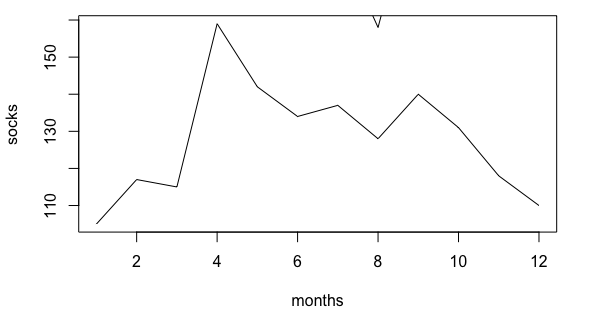
\includegraphics[width=0.7\textwidth]{plot.png}
\end{center}
\begin{enumerate}
  \item You expected to see a line for socks and a line for computers. Why is this not the case? What can you do to make both lines visible? [4 pts]

  {\color{blue} The line for computers is drawn, but it is almost entirely outside the range of the $y$ axis. To fix it we need to use the \texttt{ylim} argument to \texttt{plot()} to include the computer data.}
  \item List some other ways the plot could be improved. What needs to be done before showing it to your boss? [4 pts]

  {\color{blue} At minimum, students should say that they would add some way to differentiate between the two lines (line type or color), and a legend to tell which is which. I hope they also say make better labels (y should be ``quantity'', x should have the month names instead of numbers), a descriptive title, etc.}
\end{enumerate}

\end{enumerate}

\end{document}
\grid
